% Chase Lotito - ECE426 HW 5 - Latex

\documentclass{article}

\title{ECE426 - Homework 5}
\author{Chase Lotito - SIUC Undergraduate}
\date{}

%% PACKAGES %%

\usepackage{amsmath, amsfonts, amssymb, amsthm}
\usepackage{braket}
\usepackage{listings}
\usepackage{geometry}
\usepackage{xcolor}
\usepackage{textcomp}
\usepackage{graphicx}
\usepackage{fancyhdr}
\usepackage{sourcecodepro}
\usepackage{multirow}

%%%%%%%%%%%%%%

\graphicspath{{./images}}
\setlength\parindent{0pt}       % globally supress indentation

%% LISTINGS CONFIG %%

\definecolor{purple2}{RGB}{153,0,153} % there's actually no standard purple
\definecolor{green2}{RGB}{0,153,0} % a darker green

\lstset{
  language=Verilog,                   % the language
  basicstyle=\normalsize\ttfamily,   % size of the fonts for the code
  frame = single,
  % Color settings to match IDLE style
  keywordstyle=\color{orange},       % core keywords
  keywordstyle={[2]\color{purple2}}, % built-ins
  stringstyle=\color{green2},%
  showstringspaces=false,
  commentstyle=\color{red},%
  upquote=true,                      % requires textcomp
  numbers=left,
  breaklines=true,
}

\begin{document}

%%%%%%%%%%%%%%%%%%%%%
\pagestyle{fancy}

\maketitle

% attempt to make nice header
\fancyhead{}
\fancyhead[CH]{\normalsize{SOUTHERN ILLINOIS ECE / Chase Lotito / Spring 2024}}

%% THE HOMEWORK BEGINS HERE %%

\section{Question 1.}

Design a Mealy-type FSM that can act as a sequence detector. Complete the state table, and then simulate the FSM with Verilog behavioral-level modelling.

\bigskip

\textbf{Solution.}

\begin{table}[!h]
  \centering
  \begin{tabular}{|c|c|c|c|c|}
    \hline
    \multirow{2}{*}{\textbf{Present State}} & \multicolumn{2}{|c|}{\textbf{Next State}} & \multicolumn{2}{|c|}{\textbf{Output}} \\
    \cline{2-5}
    & w = 0 & w = 1 & w = 0 & w = 1  \\
    \hline
    A & B & C & 0 & 0 \\
    \hline
    B & B & C & 1 & 0 \\
    \hline
    C & B & C & 0 & 1 \\
    \hline
  \end{tabular}
  \caption{Mealy FSM State Table}
  \label{tab:q1-state-table}
\end{table}

The code for the Mealy FSM module.

\begin{lstlisting}[caption = "q1.v"]
// Chase Lotito - SIUC Undergraduate - Spring 2024
// ECE426 w/ Chao Lu
// HW5
// Q1: Design a Mealy-type FSM that cdan act as a sequence detector.

`timescale 1us / 1us

module mealyFSM (
    clk, reset, w, out
);

// I/O
input clk, reset, w;
output out;             // wire for continuous assignment

reg [1:0] present, next; // p for present-state, n for next-state

// Parameters for cases
// 3 cases, so lets use 2-bits
parameter A = 2'b01, B = 2'b10, C = 2'b11;  // we will count 1, 2, 3 
// Initial Conditions
initial begin
    present = A;
end

// Console log
always @ (w, out) begin
    $monitor("[PRESENT] = %d | [NEXT] = %d, w = %b | [OUTPUT] = %b \n", present, next, w, out);
end

// Next-State Combinational Logic
always @ (w, present) begin
    case (present)
        A: next = w ? C : B;
        B: next = w ? C : B;
        C: next = w ? C : B;
        default: next = 2'bxx;
    endcase
end

// Sequential Logic
// using posedge reset because not specified in problem statement.
always @ (posedge clk, posedge reset) begin
    if (reset == 1'b1)
        present <= A;
    else
        present <= next;
end

// Output Logic
assign out = ( (present == B) && (w == 1'b0) ) || ( (present == C) && (w == 1'b1) );

endmodule
\end{lstlisting}

The code for the testbench.

\begin{lstlisting}[caption = "tb.v (for q1)"]
// Chase Lotito - SIUC Undergraduate - Spring 2024
// ECE426 w/ Chao Lu
// HW5
// testbench for Q1


`include "q1.v"
`timescale 1us / 1us

module testbench();

// GTKWAVE
initial begin : GTKWAVE
    $dumpfile("q1.vcd");
    $dumpvars(0, testbench);
end

// I/O
wire out;
reg reset, clk, w;

// Initial Conditions
initial begin : initalConditions
    clk = 0;
    reset = 0;
    w = 0;
end

// Clock
always begin
    #10 clk = ~clk;
end

// Stimulus
initial begin : Stimulus
    repeat(20)
        w = #10 ~w;

    reset <= #50 1'b1;
    #100 $finish;
end

// Instantiate the FSM
mealyFSM U1 (
    .clk(clk),
    .reset(reset),
    .w(w),
    .out(out)
);

endmodule
\end{lstlisting}

\begin{figure}[!ht] 
    \centering
    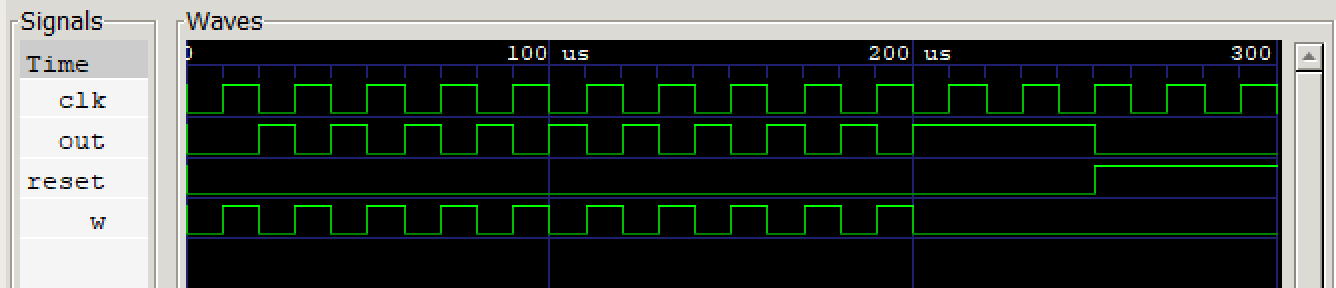
\includegraphics[width = 15cm]{q1-waves.png}
    \caption{Mealy FSM Signals}
    \label{fig:q1-waves}
\end{figure}

The terminal output from the FSM simulation is shown below in Fig. \ref{fig:q1-output}. The parameters A, B, and C are detected as 1, 2, and 3, respectively. Even though the next state might say a different value as the next line's present state, this is fine because each line does not occur for a positive edge clock cycle. 

\begin{figure}[!ht] 
    \centering
    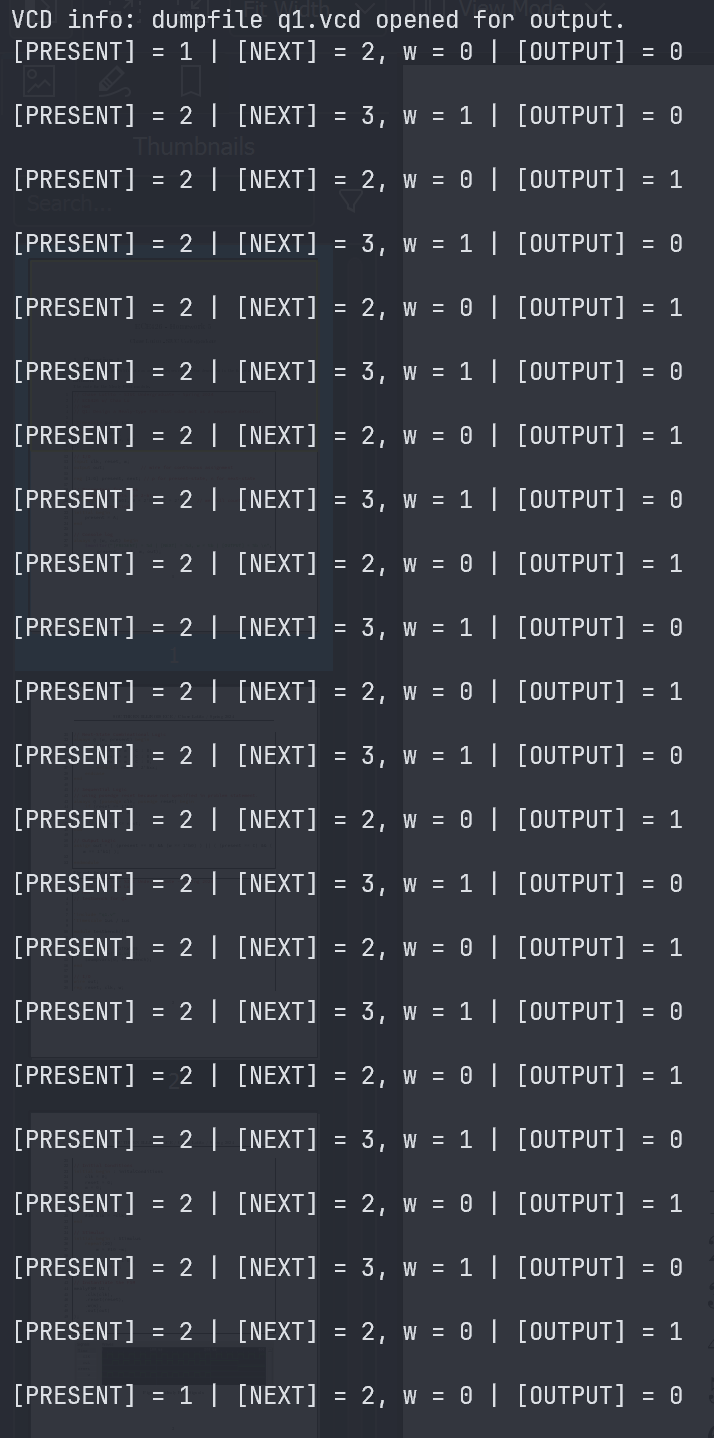
\includegraphics[width = 7cm]{q1-output.png}
    \caption{Mealy FSM Log}
    \label{fig:q1-output}
\end{figure}

\clearpage % makes a new page!!!!!!

\section{Question 2.}

Implement the FSM in Fig. \ref{fig:q2-circuit}. Show the code and part your simulation showing the correct operation of this FSM.


\begin{figure}[!ht] 
    \centering
    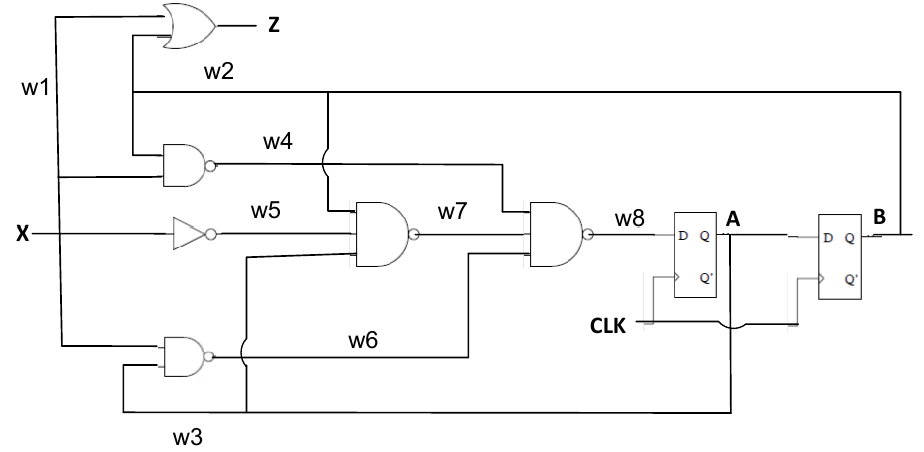
\includegraphics[width = 7cm]{q2-circuit.png}
    \caption{Q2 FSM Circuit}
    \label{fig:q2-circuit}
\end{figure}

\textbf{Solution.}

\begin{lstlisting}[caption="q2.v"]
// Chase Lotito - SIUC Undergraduate - Spring 2024
// ECE426 w/ Chao Lu
// HW5
// Q2: Code FSM from circuit diagram

`timescale 1us / 1us

// The FSM
module fsm(
    clk, z, x
);

// I/O
input clk, x;
output z;
reg A, B;

// Intermediate wires (w1 == x, w2 == B, A == A)
wire w4, w5, w6, w7, w8;

// -- Gate-Level Modelling --
// level 1
not not1(w5, x);
or or1(z, x, B);
nand nand1(w4, x, B);
nand nand2(w6, x, A);
// level 2
nand nand3(w7, B, w5, A);
// level 3
nand nand4(w8, w4, w7, w6);
//---------------------------
// -- DFFs ------------------
initial begin
    A = 0;
    B = 0;
end
always @ (posedge clk) begin
    A <= w8;
    B <= A;
end
// --------------------------
initial begin
    $monitor("[%0t us] x = %d, z = %b, w8 = %b, A = %b, B = %b", $time, x, z, w8, A, B);
end
endmodule
\end{lstlisting}

\begin{lstlisting}[caption = "tb.v (for q2)"]
// Chase Lotito - SIUC Undergraduate - Spring 2024
// ECE426 w/ Chao Lu
// HW5
// testbench for Q2
`include "q2.v"
`timescale 1us / 1us

module testbench();

// GTKWAVE
initial begin : GTKWAVE
    $dumpfile("q2.vcd");
    $dumpvars(0, testbench);
end

//--------------------------
// I/O
reg clk, x;
wire z;

// Initals
initial begin : initalConditions
   clk = 0;
   x = 0;
end

// CLOCK
always begin : clock
   #10 clk = ~clk;
end

// PROGRAM LIFETIME
initial begin : programLifeTime
    #100 $finish;
end

// STIMULUS
initial begin : stimmychecks
    repeat(20)
        x = #3 ~x;
end

// MODULE INSTANTIATION
fsm U1 (
    .clk(clk),
    .z(z),
    .x(x)
);

endmodule
\end{lstlisting}

A problem that I came across becomes clear in the simulation. For the first D-Flip-Flop to get an input of 1, then the next-state combinational logic requires x to equal 0 and 1, simultaneously. So, A and B stay at 0 for the entire simulation. 

\begin{figure}[!ht] 
    \centering
    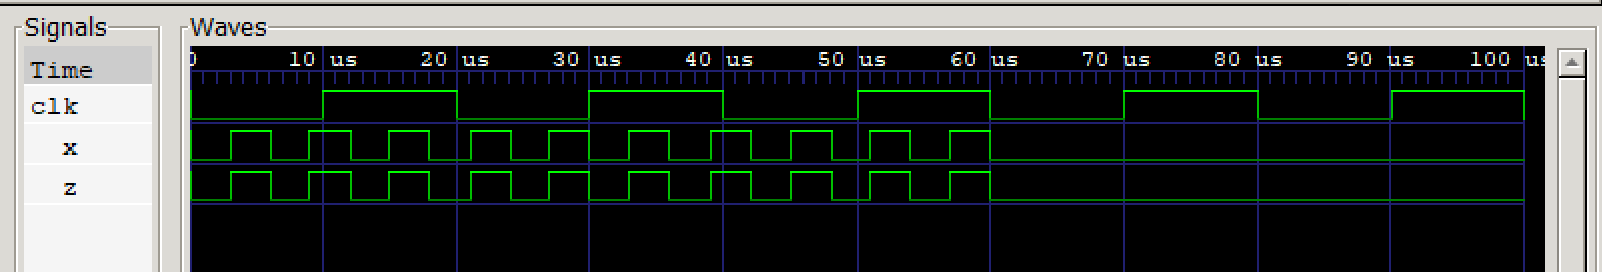
\includegraphics[width = 15cm]{q2-waves.png}
    \caption{Q2 FSM Signals}
    \label{fig:q2-waves}
\end{figure}

\begin{figure}[!ht] 
    \centering
    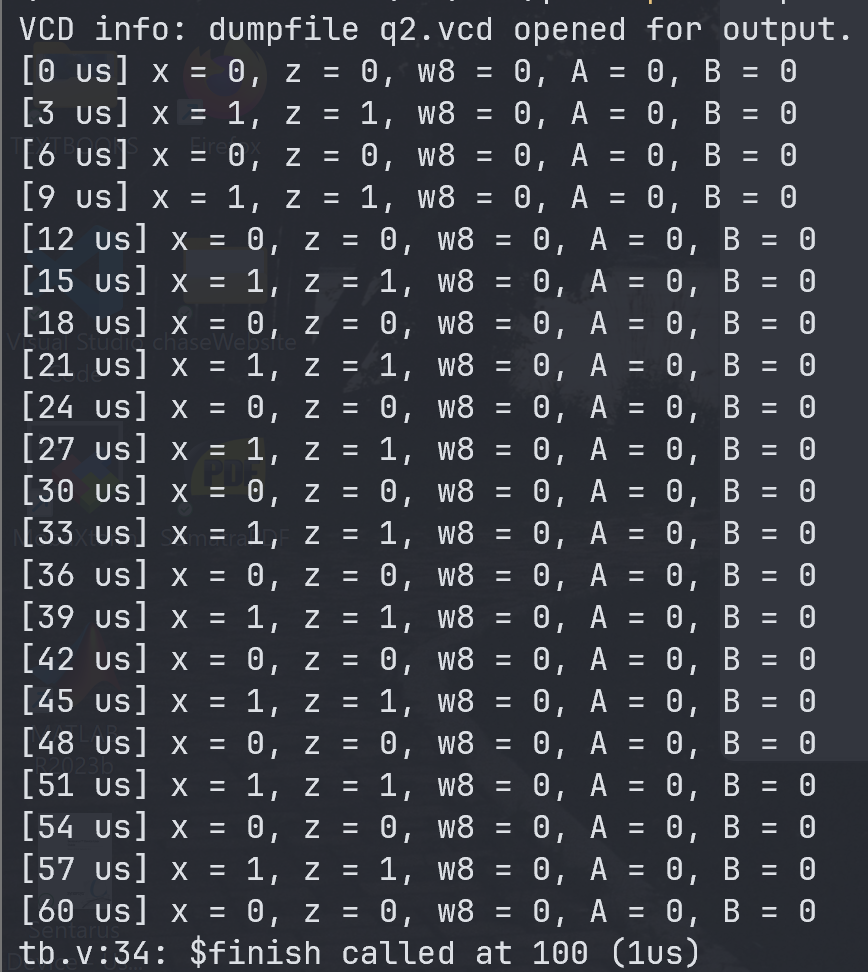
\includegraphics[width = 7cm]{q2-output.png}
    \caption{Q2 FSM Log}
    \label{fig:q2-output}
\end{figure}

\end{document}
